\newif\ifalone
\alonefalse
\ifalone
\documentclass{article}
\usepackage{graphicx}
\usepackage{natbib}
\usepackage{amsfonts}
\usepackage{amssymb}
\usepackage{amsthm}
\usepackage{bm}
\usepackage{Sweave}
\usepackage{lscape}
\usepackage{makeidx}
\usepackage{color}


\title{Categorical Random Interactions}

\author{Jarrod Hadfield (\texttt{j.hadfield@ed.ac.uk})}
\begin{document}
\maketitle
\else
\chapter{Categorical Random Interactions}
\label{chap3}
\fi



Random effect specification is a common cause of confusion, especially when we want to form interactions in the random terms. To illustrate the possibilities we'll use data collected on blue tits.

\begin{Schunk}
\begin{Sinput}
> data(BTdata)
\end{Sinput}
\end{Schunk}

The data are morphological measurements (\texttt{tarsus} length and \texttt{back} colour) made on 828 blue tit chicks from 106 mothers (\texttt{dam}). Half the offspring from each mother were swapped with half the offspring from another mother soon after hatching. The nest they were reared in is recorded as \texttt{fosternest}.  

\begin{Schunk}
\begin{Sinput}
> prior = list(R = list(V = 1, nu = 0.002), G = list(G1 = list(V = 1, 
+     nu = 0.002), G2 = list(V = 1, nu = 0.002)))
> m3a.1 <- MCMCglmm(tarsus ~ sex, random = ~dam + fosternest, data = BTdata, 
+     verbose = FALSE, prior = prior)
\end{Sinput}
\end{Schunk}

fits \texttt{sex} as a fixed effect, and \texttt{dam} and \texttt{fosternest} as random effects.  

\begin{Schunk}
\begin{Sinput}
> diag(autocorr(m3a.1$VCV)[2, , ])
\end{Sinput}
\begin{Soutput}
        dam  fosternest       units 
0.074601677 0.381514717 0.003330548 
\end{Soutput}
\begin{Sinput}
> plot(m3a.1$VCV)
\end{Sinput}
\end{Schunk}

\begin{figure}[!h]
\begin{center}
\begin{Schunk}
\begin{Soutput}
        dam  fosternest       units 
0.074601677 0.381514717 0.003330548 
\end{Soutput}
\end{Schunk}
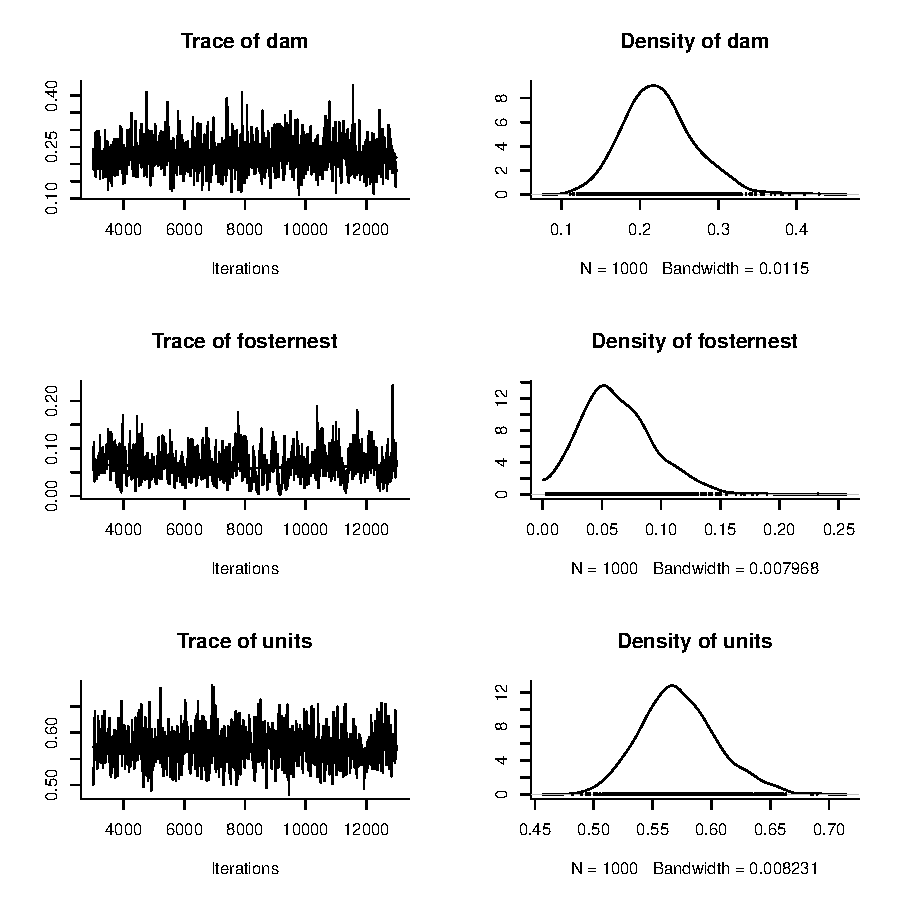
\includegraphics{Lecture3-005}
\end{center}
\caption{MCMC summary plot for the variance components from model \texttt{m3a.1}.}
\label{mBTVCV-fig}
\end{figure}

Perhaps the autocorrelation for the \texttt{fosternest} variance is a little higher than we would like, and so we may like to run it for longer.

\begin{Schunk}
\begin{Sinput}
> effectiveSize(m3a.1$VCV)
\end{Sinput}
\begin{Soutput}
       dam fosternest      units 
  915.6996   447.2382   944.6921 
\end{Soutput}
\end{Schunk}

Indeed, we've only sampled the fosternest variance about half as well as the other two variance components.\\

The posterior correlation between the parameters is low

\begin{Schunk}
\begin{Sinput}
> cor(m3a.1$VCV)
\end{Sinput}
\begin{Soutput}
                   dam fosternest       units
dam         1.00000000 -0.2179331 -0.03701361
fosternest -0.21793311  1.0000000 -0.15619239
units      -0.03701361 -0.1561924  1.00000000
\end{Soutput}
\end{Schunk}

which is not that surprising give the data come from an experiment which was designed in order to estimate these variance components. In general, variance components will show negative posterior correlations because the the total variance is being divided up. Imagine cutting a piece of string; making one bit longer has to reduce the size of the other bits, by necessity. If we hadn't experimentally manipulated the birds then all chicks with the same mother, would be raised in the same nest, and there would be no information in the data to separate these terms. In this case the posterior correlation between these parameters would approach -1 as the prior information goes to zero.\\  

The lower 95\% credible interval for the \texttt{fosternest} variance is low

\begin{Schunk}
\begin{Sinput}
> HPDinterval(m3a.1$VCV)
\end{Sinput}
\begin{Soutput}
                 lower     upper
dam        0.139813978 0.3215853
fosternest 0.008835799 0.1204842
units      0.507523214 0.6318353
attr(,"Probability")
[1] 0.95
\end{Soutput}
\end{Schunk}

and perhaps a model without it would be better supported, although the DIC suggest not:

\begin{Schunk}
\begin{Sinput}
> priorb <- prior
> priorb[[2]] <- priorb[[2]][-2]
> m3a.2 <- MCMCglmm(tarsus ~ sex, random = ~dam, data = BTdata, 
+     verbose = FALSE, prior = priorb)
> m3a.2$DIC
\end{Sinput}
\begin{Soutput}
[1] 2014.393
\end{Soutput}
\begin{Sinput}
> m3a.1$DIC
\end{Sinput}
\begin{Soutput}
[1] 1991.861
\end{Soutput}
\end{Schunk}


The tarsus lengths were standardised prior to analysis - this is not recommended, but was done in the original analyses of these data \citep{Hadfield.2007} so that comparisons would be scale invariant. The original analyses were done in REML where it is hard to get accurate confidence intervals for functions of variance components.  With MCMC procedures this is simple. For example if we want to know what proportion of the total variance is explained by dams 

\begin{Schunk}
\begin{Sinput}
> HPDinterval(m3a.1$VCV[, 1]/rowSums(m3a.1$VCV))
\end{Sinput}
\begin{Soutput}
        lower     upper
var1 0.180847 0.3524168
attr(,"Probability")
[1] 0.95
\end{Soutput}
\end{Schunk}

One nice thing though about standardised data is that effect sizes are immediately apparent. For example, fixed effects are in standard deviation units and the sex effects are non-trivial:

\begin{Schunk}
\begin{Sinput}
> summary(m3a.1$Sol)
\end{Sinput}
\begin{Soutput}
Iterations = 3001:12991
Thinning interval = 10 
Number of chains = 1 
Sample size per chain = 1000 

1. Empirical mean and standard deviation for each variable,
   plus standard error of the mean:

               Mean      SD Naive SE Time-series SE
(Intercept) -0.4077 0.06661 0.002106       0.002399
sexMale      0.7707 0.05751 0.001819       0.001764
sexUNK       0.2029 0.12757 0.004034       0.004139

2. Quantiles for each variable:

                2.5%     25%     50%     75%   97.5%
(Intercept) -0.53484 -0.4539 -0.4092 -0.3636 -0.2648
sexMale      0.66454  0.7308  0.7717  0.8082  0.8852
sexUNK      -0.04425  0.1178  0.2045  0.2880  0.4484
\end{Soutput}
\end{Schunk}

Given that the sexes differ in their mean phenotype it may be worth exploring whether they vary in other ways. For example, perhaps there are sex-limited genes that mean that related brothers resemble each other more than they do their sisters. Perhaps females are less sensitive to environmental variation? To fit these models it will be necessary to understand how the variance functions, such as \texttt{us()} and \texttt{idh()}, work.  We could refit the model \texttt{m3a.1} using the random effect specifications:

\begin{Schunk}
\begin{Sinput}
> random = ~us(1):dam + us(1):fosternest
\end{Sinput}
\end{Schunk}

\begin{Schunk}
\begin{Sinput}
> random = ~idh(1):dam + idh(1):fosternest
\end{Sinput}
\end{Schunk}

and these would give exactly the same answer as the model specified as $^{\sim}$\texttt{dam+fosternest}. The term inside the brackets is a model formula and is interpreted exactly how you would interpret any R formula expect the intercept is not fitted by default. These formula are therefore fitting an intercept which is interacted with the random effects. For the dam terms we can get a representation of the interaction for the first few levels of \texttt{dam}:

\begin{Schunk}
\begin{Sinput}
> levels(BTdata$dam)[1:5]
\end{Sinput}
\begin{Soutput}
[1] "Fem2"    "Fem20"   "Fem3"    "Fem5"    "K983388"
\end{Soutput}
\end{Schunk}


\begin{displaymath}
\begin{array}{c|rrrrrc}
&{\color{red} \texttt{Fem2}}&{\color{red} \texttt{Fem20}}&{\color{red} \texttt{Fem3}}&{\color{red} \texttt{Fem5}}&{\color{red} \texttt{K983388}}&\dots\\
\hline\\
{\color{blue} \texttt{1}}&{\color{blue} \texttt{1}}.{\color{red} \texttt{Fem2}}&{\color{blue} \texttt{1}}.{\color{red} \texttt{Fem20}}&{\color{blue} \texttt{1}}.{\color{red} \texttt{Fem3}}&{\color{blue} \texttt{1}}.{\color{red} \texttt{Fem5}}&{\color{blue} \texttt{1}}.{\color{red} \texttt{K983388}}&\dots\\
\end{array}
\end{displaymath}
  
Across the top, we have the original dam effects in red, and along the side we have the term defined by the variance structure formula (just the intercept in this case).  The interaction forms a new set of factors. Although they have different names from the original \texttt{dam} levels it is clear that there is a one to one mapping between the original and the new factor levels and the models are therefore equivalent.  For more complex interactions this is not the case.\\

We could also fit \texttt{sex} in the variance structure model, (i.e. \texttt{us({\color{blue}sex}):{\color{red}dam}} or \texttt{idh({\color{blue}sex}):{\color{red}dam}})\footnote{Remember that a global intercept is not fitted by default for variance structure models, and the model formula is essentially $^{\sim}$\texttt{sex-1}. To add the global intercept, \texttt{us({\color{blue}1+sex}):{\color{red}dam}} could be fitted but this can be harder to interpret because the effects are then {\color{blue} \texttt{Fem}}, {\color{blue} \texttt{Male-Fem}} and {\color{blue} \texttt{UNK-Fem}}. If a \texttt{us} structure is fitted, the two models are equivalent reparameterisations of each other although the priors have to modified accordingly. This is not the case if the variance function is \texttt{idh}. In this case the sex-specific variances are allowed to vary as before, but a constant covariance equal to $\sigma^{2}_{\color{blue} \texttt{Fem}}$ is also assumed}:

\begin{displaymath}
\begin{array}{c|rrrrrc}
&{\color{red} \texttt{Fem2}}&{\color{red} \texttt{Fem20}}&{\color{red} \texttt{Fem3}}&{\color{red} \texttt{Fem5}}&{\color{red} \texttt{K983388}}&\dots\\
\hline\\
{\color{blue} \texttt{Fem}}&{\color{blue} \texttt{Fem}}.{\color{red} \texttt{Fem2}}&{\color{blue} \texttt{Fem}}.{\color{red} \texttt{Fem20}}&{\color{blue} \texttt{Fem}}.{\color{red} \texttt{Fem3}}&{\color{blue} \texttt{Fem}}.{\color{red} \texttt{Fem5}}&{\color{blue} \texttt{Fem}}.{\color{red} \texttt{K983388}}&\dots\\
{\color{blue} \texttt{Male}}&{\color{blue} \texttt{Male}}.{\color{red} \texttt{Fem2}}&{\color{blue} \texttt{Male}}.{\color{red} \texttt{Fem20}}&{\color{blue} \texttt{Male}}.{\color{red} \texttt{Fem3}}&{\color{blue} \texttt{Male}}.{\color{red} \texttt{Fem5}}&{\color{blue} \texttt{Male}}.{\color{red} \texttt{K983388}}&\dots\\
{\color{blue} \texttt{UNK}}&{\color{blue} \texttt{UNK}}.{\color{red} \texttt{Fem2}}&{\color{blue} \texttt{UNK}}.{\color{red} \texttt{Fem20}}&{\color{blue} \texttt{UNK}}.{\color{red} \texttt{Fem3}}&{\color{blue} \texttt{UNK}}.{\color{red} \texttt{Fem5}}&{\color{blue} \texttt{UNK}}.{\color{red} \texttt{K983388}}&\dots\\
\end{array}
\end{displaymath}

which creates three times as many random factors, one associated with offspring of each sex for each each dam.  

\section{\texttt{idh} Variance Structure}

The different variance functions make different assumptions about how the effects associated with these different factors are distributed. First, we may want to allow the variance in the effects to be different for each row of factors; i.e. does the identity of a chicks mother explain different amounts of variation depending on the sex of the chick. We can fit this model using the \texttt{idh} function and represent our belief in how the effects are distributed as a $3\times3$ covariance matrix ${\bf V}$:    

\begin{displaymath}
{\bf V}_{{\color{red} \texttt{dam}}}=
\left[
\begin{array}{ccc}
\sigma^{2}_{\color{blue}\texttt{Female}}&0&0\\
0&\sigma^{2}_{\color{blue}\texttt{Male}}&0\\
0&0&\sigma^{2}_{\color{blue}\texttt{UNK}}\\
\end{array}
\right]
\end{displaymath}

In the simpler models we had fitted in Lectures \ref{chap1} and \ref{chap2} ${\bf V}$ was a scalar (${\bf V} = \sigma^{2}$) rather than a matrix, and the prior specification was relatively simple.  We will come back to prior specifications for covariance matrices in Section \ref{VCVprior-sec}, but for now note that the prior for the dam component has \texttt{V} as a $3\times3$ identity matrix:  

\begin{Schunk}
\begin{Sinput}
> priorb = list(R = list(V = diag(1), nu = 0.002), G = list(G1 = list(V = diag(3), 
+     nu = 2.002), G2 = list(V = 1, nu = 0.002)))
> m3a.3 <- MCMCglmm(tarsus ~ sex, random = ~idh(sex):dam + fosternest, 
+     data = BTdata, verbose = FALSE, prior = priorb)
\end{Sinput}
\end{Schunk}


\begin{figure}[!h]
\begin{center}
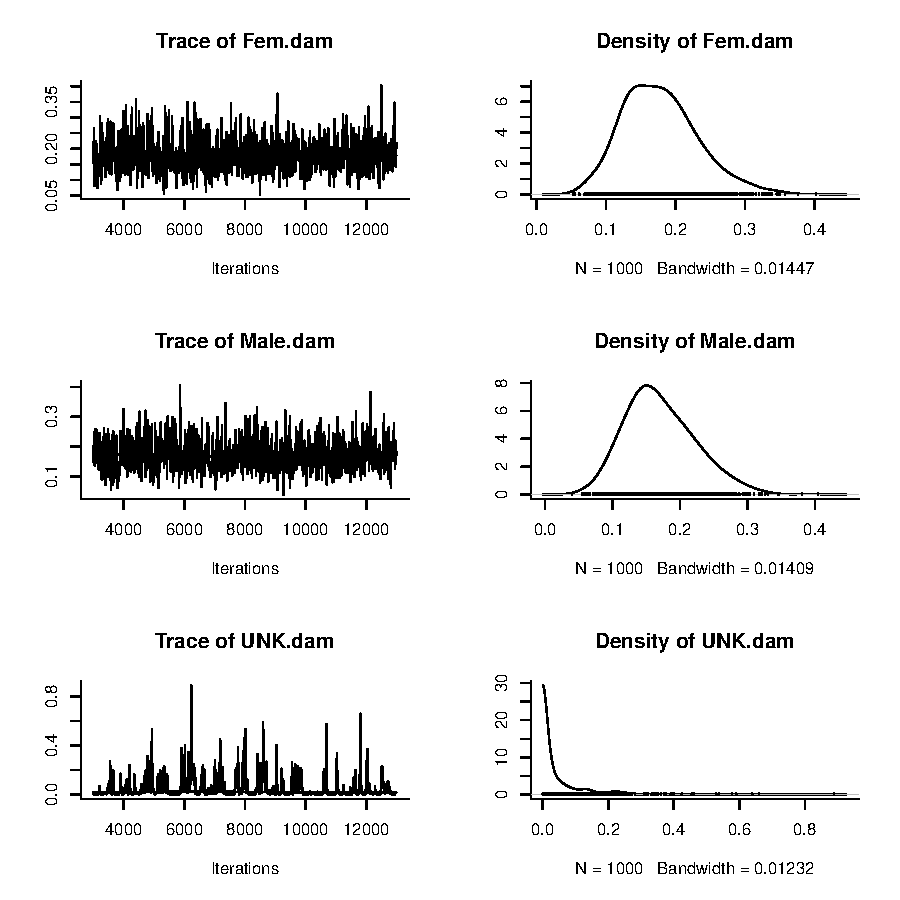
\includegraphics{Lecture3-018}
\end{center}
\caption{MCMC summary plot for the sex-specific dam variance components from model \texttt{m3a.3}. The number of chicks with unknown (\texttt{UNK}) sex is low, with very little replication within dams. The posterior distribution for the \texttt{UNK} variance component is dominated by the prior which has a marginal distribution of \texttt{V=1} and \texttt{nu=0.002}.}
\label{BTidh-fig}
\end{figure}

The sex specific variances for males and females look pretty similar, but the sex-specific variance for birds with unknown sex is not behaving well. This is not that surprising given that there are only 47 birds with unknown sex and these tend to be thinly spread across dams. This variance component is likely to be dominated by the prior, but for now we'll leave the model as it is and come back to some possible alternative solutions later.\\

We can extract the marginal means for each variance and place them into a matrix:

\begin{Schunk}
\begin{Sinput}
> Vdam.3 <- diag(colMeans(m3a.3$VCV)[1:3])
> colnames(Vdam.3) <- colnames(m3a.3$VCV)[1:3]
> Vdam.3
\end{Sinput}
\begin{Soutput}
       Fem.dam  Male.dam   UNK.dam
[1,] 0.2499392 0.0000000 0.0000000
[2,] 0.0000000 0.2371669 0.0000000
[3,] 0.0000000 0.0000000 0.3781115
\end{Soutput}
\end{Schunk}

Note, that they are in general less than the marginal mean of the dam variance in model \texttt{m3a.1} (0.226)  where a sex interaction was not fitted.  Because the dam effects are assumed to be multivariate normal we can plot an ellipsoid that completely represents their distribution (you can rotate the figure in R):

\begin{Schunk}
\begin{Sinput}
> plotsubspace(Vdam.3, axes.lab = TRUE)
\end{Sinput}
\end{Schunk}

If we had measured the offspring of a lot of dams, and for each dam we had measured a very large number of offspring of each sex, then we could calculate the average tarsus lengths within a nest for males, females and unknowns separately. If we produced a scatter plot of these means the data would have the same shape as this ellipsoid and 95\% of the data would lie inside.

\begin{figure}[!h]
\begin{center}
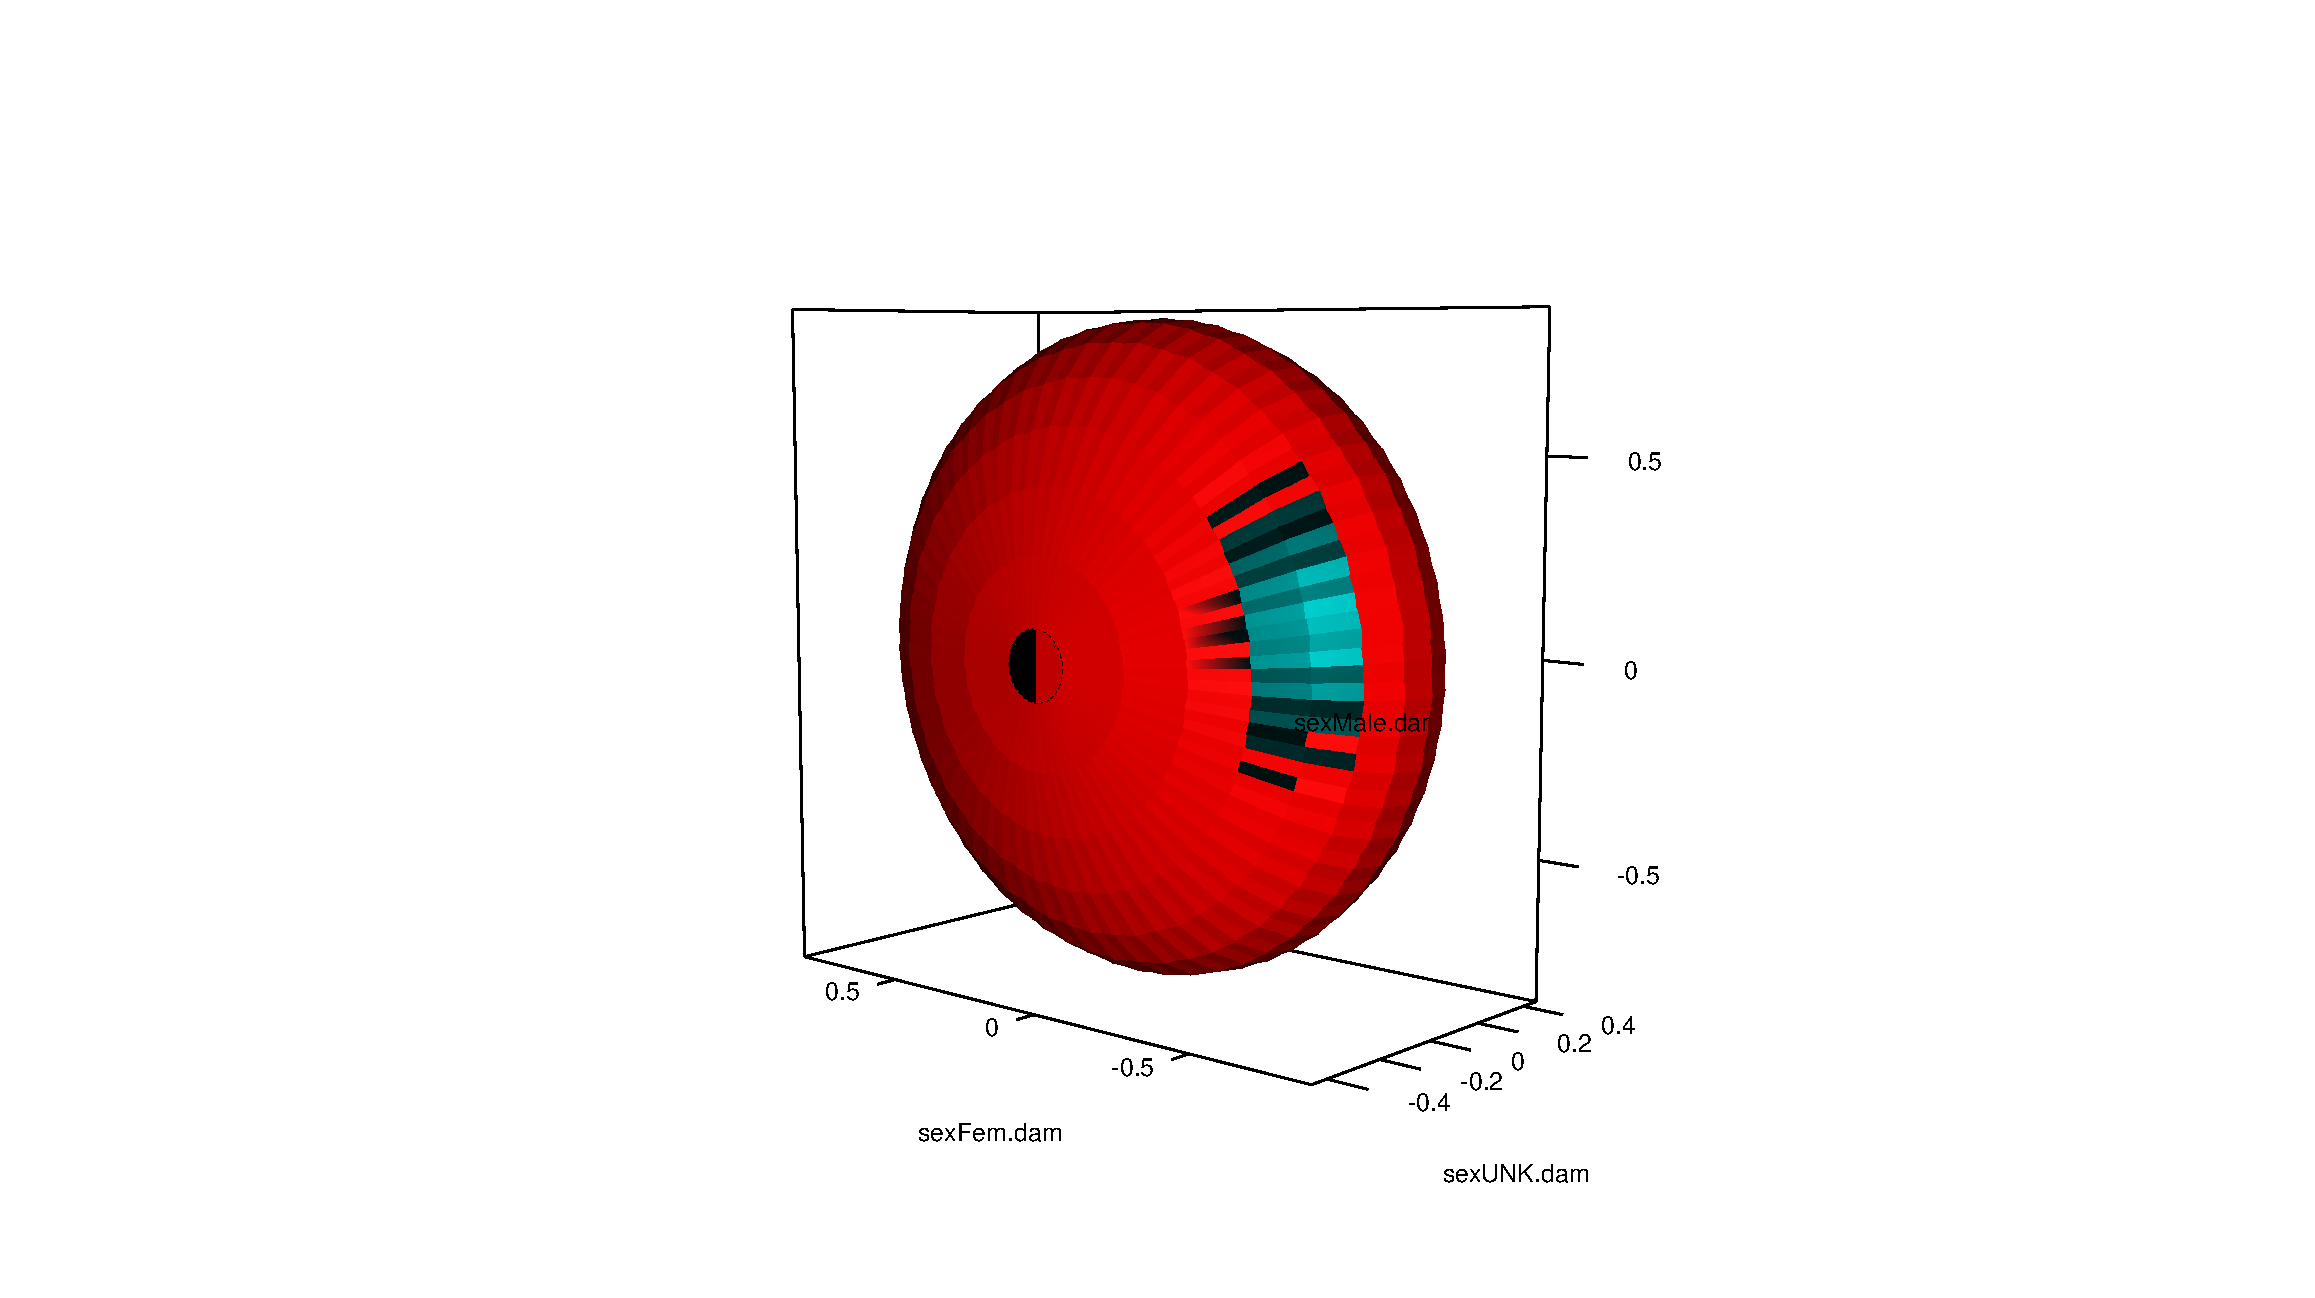
\includegraphics{rgl1.pdf}
\end{center}
\caption{Ellipsoid that circumscribes 95\% of the expected dam effects as estimated in model \texttt{m3a.3}. This can be thought of as a scatter plot of the dam effects between each sex, if the dam effects could be directly measured.  Because the covariances of the dam effects between the sexes were set to zero the axes of the ellipsoids are all parallel to the figure axes.}
\label{rgl1-fig}
\end{figure}

\section{\texttt{us} Variance Structure}

The oddity of the model, and the meaning of the off-diagonal zeros, should become apparent. We have assumed that the different sexes with in a nest are independent. If we plotted the average tarsus lengths for males against the average tarsus lengths for females for each dam this model implies we should see no relationship. We can relax this assumption using the \texttt{us} function which estimates the matrix: 

\begin{displaymath}
{\bf V}_{{\color{red} \texttt{dam}}}=
\left[
\begin{array}{ccc}
\sigma^{2}_{\color{blue}\texttt{Female}}&\sigma_{\color{blue}\texttt{Female}, \texttt{Male}}&\sigma_{\color{blue}\texttt{Female}, \texttt{UNK}}\\
\sigma_{\color{blue}\texttt{Female}, \texttt{Male}}&\sigma^{2}_{\color{blue}\texttt{Male}}&\sigma_{\color{blue}\texttt{Male}, \texttt{UNK}}\\
\sigma_{\color{blue}\texttt{Female}, \texttt{UNK}}&\sigma_{\color{blue}\texttt{Male}, \texttt{UNK}}&\sigma^{2}_{\color{blue}\texttt{UNK}}\\
\end{array}
\right]
\end{displaymath}

We will now use a prior for the covariance matrix where nu=4 (1 more than the dimension of {\bf V}) and the prior covariance matrix is an diagonal matrix with small variances. This may seem surprising but the motivation is laid out in Section \ref{VCVprior-sec}: 

\begin{Schunk}
\begin{Sinput}
> prior.m3a.4 = list(R = list(V = diag(1), nu = 0.002), G = list(G1 = list(V = diag(3) * 
+     0.02, nu = 4), G2 = list(V = 1, nu = 0.002)))
> m3a.4 <- MCMCglmm(tarsus ~ sex, random = ~us(sex):dam + fosternest, 
+     data = BTdata, verbose = FALSE, prior = prior.m3a.4)
\end{Sinput}
\end{Schunk}

The posterior mean (co)variances for this model show that the covariances are almost the same magnitude as the variances suggesting strong correlations: 

\begin{Schunk}
\begin{Sinput}
> Vdam.4 <- matrix(colMeans(m3a.4$VCV)[1:9], 3, 3)
> colnames(Vdam.4) <- colnames(m3a.4$VCV)[1:3]
> Vdam.4
\end{Sinput}
\begin{Soutput}
     Fem:Fem.dam Male:Fem.dam UNK:Fem.dam
[1,]   0.2334452    0.2010293   0.2264327
[2,]   0.2010293    0.2118694   0.2165657
[3,]   0.2264327    0.2165657   0.2906382
\end{Soutput}
\end{Schunk}

The distribution of dam effects in this model looks substantially different (Figure \ref{rgl2-fig}):

\begin{Schunk}
\begin{Sinput}
> plotsubspace(Vdam.4, axes.lab = TRUE, wire.frame = T)
\end{Sinput}
\end{Schunk}

\begin{figure}[!h]
\begin{center}
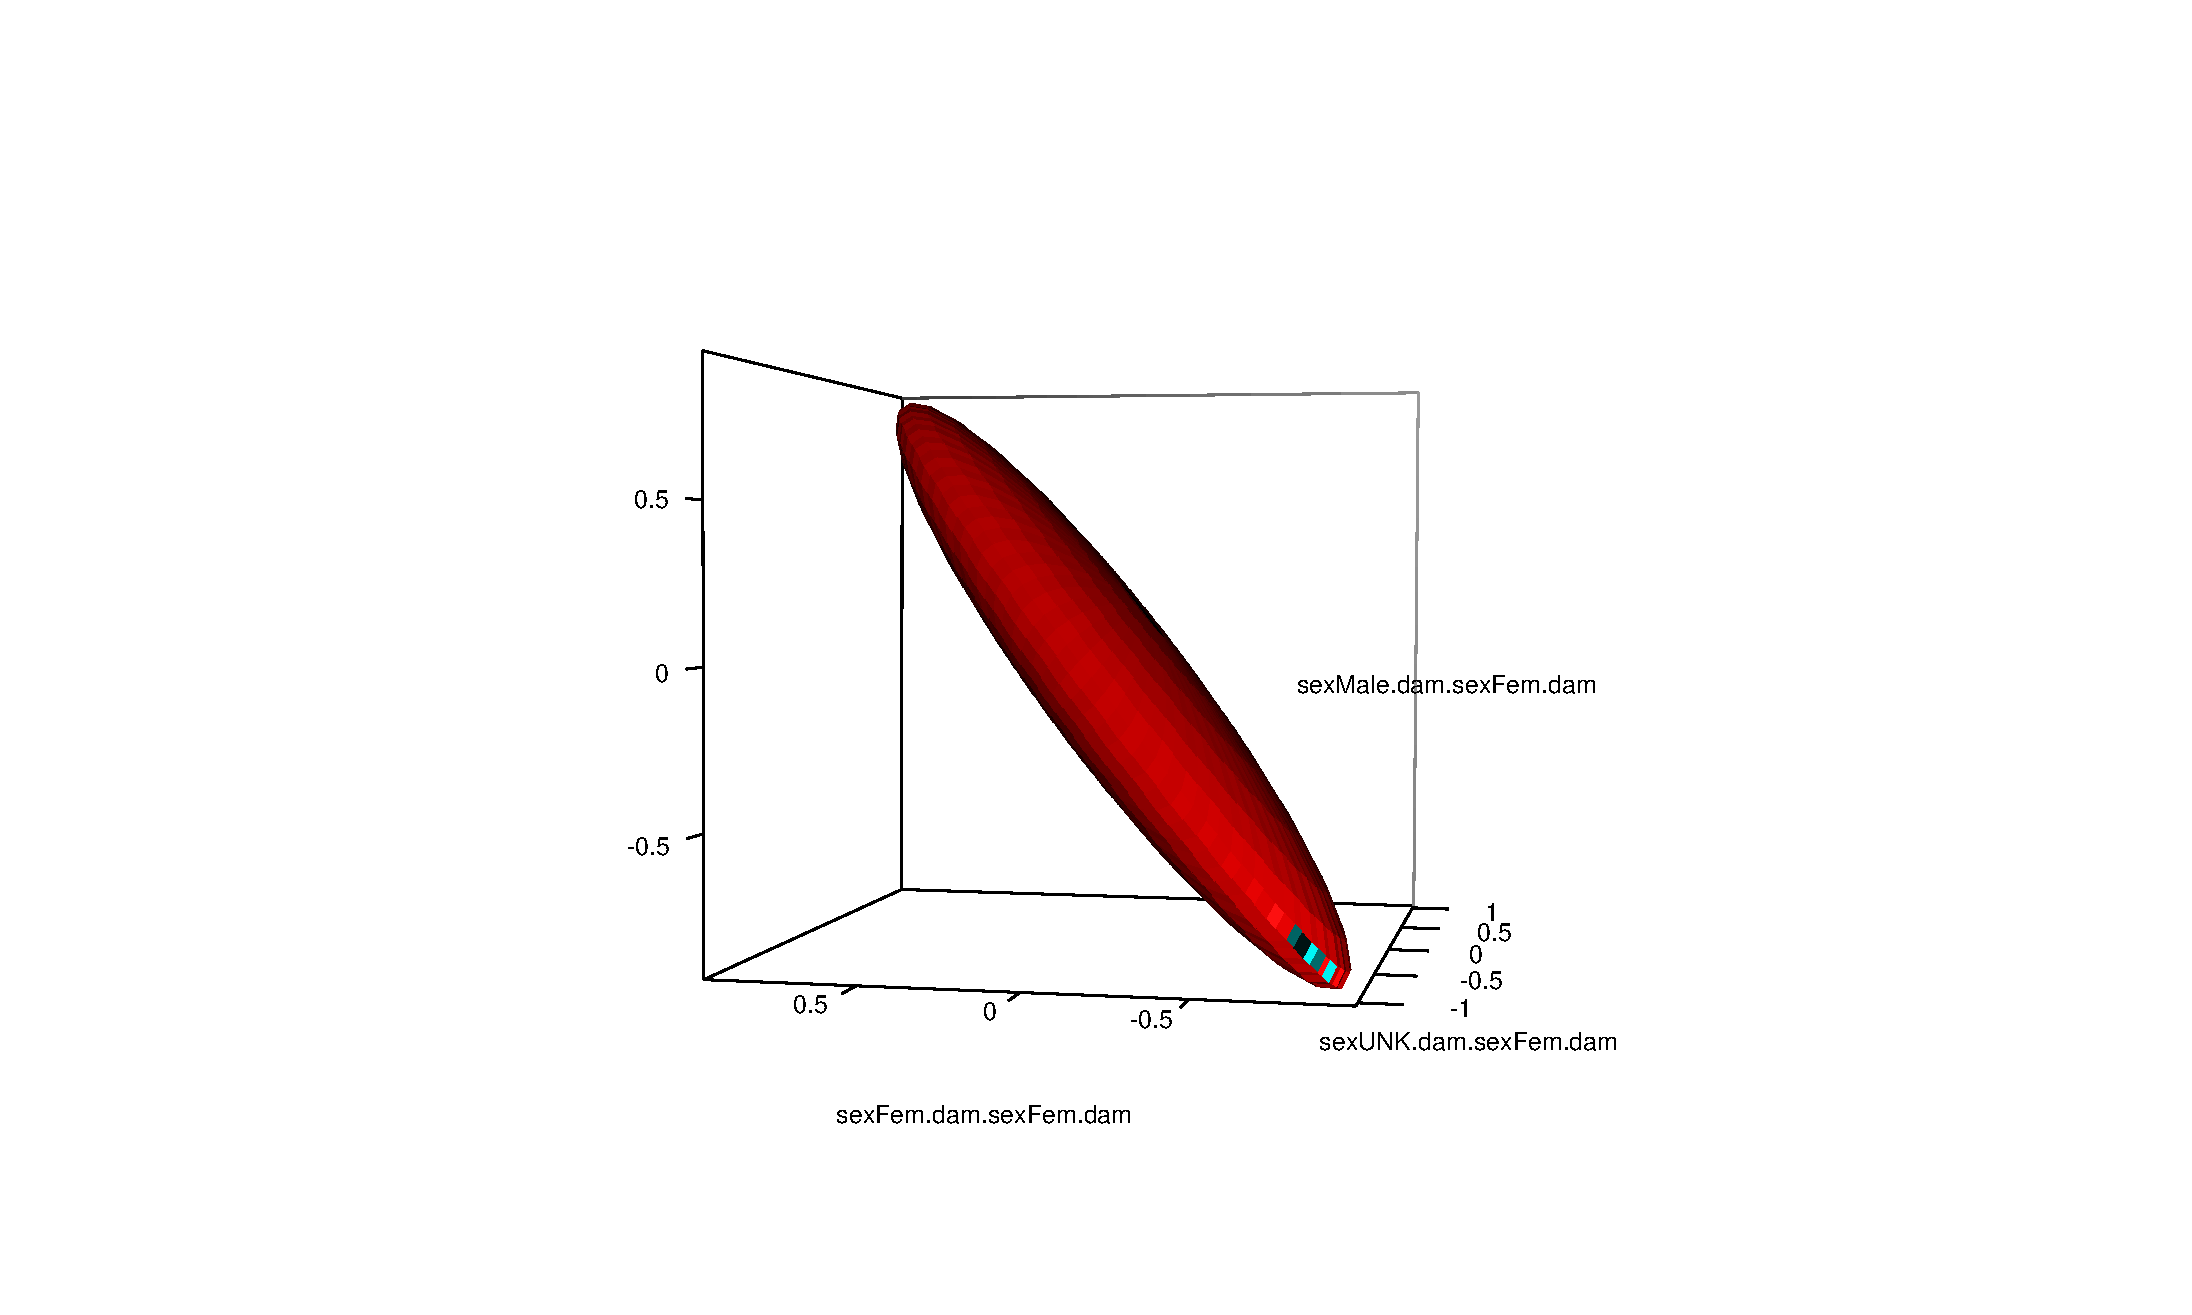
\includegraphics{rgl2.pdf}
\end{center}
\caption{Ellipsoid that circumscribes 95\% of the expected dam effects as estimated in model \texttt{m3a.4}. This can be thought of as a scatter plot of the dam effects between each sex, if the dam effects could be directly measured.  The correlations of the dam effects between the sexes were estimated and found to be close to one, and the sex-specific variances were all roughly equal in magnitude.  Consequently the major axis of the ellipsoid lies at $45^{o}$ to the figure axes.}
\label{rgl2-fig}
\end{figure}


Covariances can be hard to interpret, and I usually find correlations easier to think about. They can also be useful for detecting problems in the chain. In model \texttt{m3a.1} the dam variance for chicks with unknown sex was behaving badly and was getting `trapped' at zero. When fitting a $2\times2$ covariance matrix similar things can happen when correlations are close to -1 and 1, and this may not be obvious from the marginal distribution of the covariances:

\begin{Schunk}
\begin{Sinput}
> plot(posterior.cor(m3a.4$VCV[, 1:9])[, c(2, 3, 7)])
\end{Sinput}
\end{Schunk}

\begin{figure}[!h]
\begin{center}
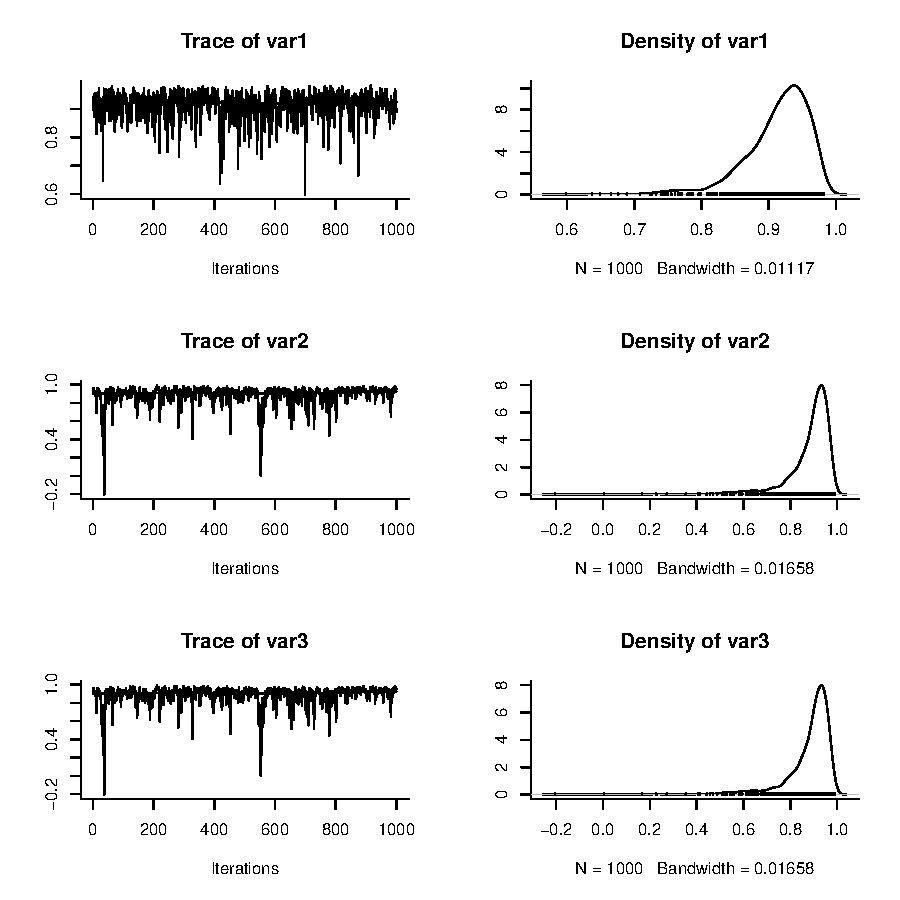
\includegraphics{Lecture3-025}
\end{center}
\caption{MCMC summary plot for the between sex correlations in dam effects from model \texttt{m3a.4}.}
\label{BTcor-fig}
\end{figure}

All the correlations are very close to one, and the variances all pretty equal so we'd probably consider the simpler model. We could try using DIC to compare models, although given the different prior specifications for the two models it is unclear whether this would be meaningful. However, the simpler model does seem to have better support as intuition suggests:

\begin{Schunk}
\begin{Sinput}
> m3a.4$DIC
\end{Sinput}
\begin{Soutput}
[1] 1996.94
\end{Soutput}
\begin{Sinput}
> m3a.1$DIC
\end{Sinput}
\begin{Soutput}
[1] 1991.861
\end{Soutput}
\end{Schunk}

\section{Compound Variance Structures}

There are also ways of specifying models that lie somewhere between the simple model (\texttt{mBT}), where dam effects are assumed to be equivalent across the sexes, and the most complex model (\texttt{mBT2}), where dam effects are allowed to vary across the sexes and covary between the sexes to different degrees. Some alternatives are listed in Table \ref{rspec}.\\

To be completed ....\\

\begin{landscape}
\begin{table}
\begin{center}
\begin{tabular}{ccccc}
\hline
\texttt{lmer} & \texttt{MCMCglmm}/\texttt{asreml}&No. Parameters&Variance&Correlation\\
\hline
\\
\texttt{(1|dam)}&\texttt{dam}&1&
$\left[
\begin{array}{ccc}
V&V&V\\
V&V&V\\
V&V&V\\
\end{array}
\right]$
&
$\left[
\begin{array}{ccc}
1&1&1\\
1&1&1\\
1&1&1\\
\end{array}
\right]$\\
\\
\texttt{(sex-1|dam)}&\texttt{us(sex):dam}&6&
$\left[
\begin{array}{ccc}
V_{1,1}&C_{1,2}&C_{1,3}\\
C_{1,2}&V_{2,2}&C_{2,3}\\
C_{1,3}&C_{2,3}&V_{3,3}\\
\end{array}
\right]$
&
$\left[
\begin{array}{ccc}
1&r_{1,2}&r_{1,3}\\
r_{1,2}&1&r_{2,3}\\
r_{1,3}&r_{2,3}&1\\
\end{array}
\right]$\\
\\
\texttt{(1|sex:dam)}&\texttt{sex:dam}&1&
$\left[
\begin{array}{ccc}
V&0&0\\
0&V&0\\
0&0&V\\
\end{array}
\right]$
&
$\left[
\begin{array}{ccc}
1&0&0\\
0&1&0\\
0&0&1\\
\end{array}
\right]$\\
\\
\texttt{(1|dam)}+\texttt{(1|sex:dam)}&\texttt{dam}+\texttt{sex:dam}&2&
$\left[
\begin{array}{ccc}
V_{1}+V_{2}&V_{1}&V_{1}\\
V_{1}&V_{1}+V_{2}&V_{1}\\
V_{1}&V_{1}&V_{1}+V_{2}\\
\end{array}
\right]$
&
$\left[
\begin{array}{ccc}
1&r&r\\
r&1&r\\
r&r&1\\
\end{array}
\right]$\\
\\
-&\texttt{idh(sex):dam}&3&
$\left[
\begin{array}{ccc}
V_{1,1}&0&0\\
0&V_{2,2}&0\\
0&0&V_{3,3}\\
\end{array}
\right]$
&
$\left[
\begin{array}{ccc}
1&0&0\\
0&1&0\\
0&0&1\\
\end{array}
\right]$\\
%-&\texttt{idh(1+sex):dam}&3&
%$\left[
%\begin{array}{ccc}
%V_{1,1}&V_{1,1}&V_{1,1}\\
%V_{1,1}&V_{1,1}+V_{2,2}&V_{1,1}\\
%V_{1,1}&V_{1,1}&V_{1,1}+V_{3,3}\\
%\end{array}
%\right]$
%&
%$\left[
%\begin{array}{ccc}
%V_{1,1}&\frac{V_{1,1}}{\sqrt{V_{1,1}(V_{1,1}+V_{2,2})}}&\frac{V_{1,1}}{\sqrt{V_{1,1}(V_{1,1}+V_{3,3})}}\\
%\frac{V_{1,1}}{\sqrt{V_{1,1}(V_{1,1}+V_{2,2})}}&V_{1,1}+V_{2,2}&\frac{V_{1,1}}{\sqrt{(V_{1,1}+V_{2,2})(V_{1,1}+V_{3,3})}}\\
%\frac{V_{1,1}}{\sqrt{V_{1,1}(V_{1,1}+V_{3,3})}}&\frac{V_{1,1}}{\sqrt{(V_{1,1}+V_{2,2})(V_{1,1}+V_{3,3})}}&V_{1,1}+V_{3,3}\\
%\end{array}
%\right]$\\
%-&\texttt{us(at.level(sex, 2)+set.level(sex, c(1, 3)):dam}&$\left[
%\begin{array}{ccc}
%V_{1,1}&C_{1,2}&C_{1,3}\\
%C_{1,2}&V_{2,2}&C_{2,3}\\
%C_{1,3}&C_{2,3}&V_{3,3}\\
%\end{array}
%\right]$
%&
%$\left[
%\begin{array}{ccc}
%1&r_{1,2}&r_{1,3}\\
%r_{1,2}&1&r_{2,3}\\
%r_{1,3}&r_{2,3}&1\\
%\end{array}
%\right]$\\
\\
-&\texttt{corh(sex):dam}&4&
$\left[
\begin{array}{ccc}
V_{1,1}&rV_{1,1}V_{2,2}&rV_{1,1}V_{2,2}\\
rV_{1,1}V_{2,2}&V_{2,2}&rV_{2,2}V_{2,3}\\
rV_{1,1}V_{3,3}&rV_{2,2}V_{3,3}&V_{3,3}\\
\end{array}
\right]$
&
$\left[
\begin{array}{ccc}
1&r&r\\
r&1&r\\
r&r&1\\
\end{array}
\right]$\\
\\
-&\texttt{cor(sex):dam}&3&
$\left[
\begin{array}{ccc}
1&r_{1,2}&r_{1,3}\\
r_{1,2}&1&r_{2,3}\\
r_{1,3}&r_{2,3}&1\\
\end{array}
\right]$
&
$\left[
\begin{array}{ccc}
1&r_{1,2}&r_{1,3}\\
r_{1,2}&1&r_{2,3}\\
r_{1,3}&r_{2,3}&1\\
\end{array}
\right]$\\
\\
\hline
\end{tabular}
\end{center}
\caption{Different random effect specifications in \texttt{lmer}, \texttt{MCMCglmm} and \texttt{asreml}. \texttt{sex} is a factor with three levels so the resulting matrix is $3\times3$. Continuous variables can also go on the LHS of the pipe, or within the variance structure functions (e.g. \texttt{us},\texttt{idh}). In this case the associated parameters are regression coefficients for which a variance is estimated. For example, if the chicks were of different ages (or we'd measured the same chicks at different ages) we may want to see if the growth rate is more similar for chicks raised by the same mother. \texttt{(1+age|dam)} or \texttt{us(1+age):dam} estimates a $2\times2$ matrix which includes the variance in intercepts (when \texttt{age}=0), the variance in slopes, and the covariance that exists between them.}
\label{rspec}
\end{table}
\end{landscape}

\section{Heterogenous Residual Variance}
\label{heter-sec}
To be started... In short - if you've fitted a sex by dam interaction I would always allow the sexes to have different residual variances. Use \texttt{idh(sex):units}.

\section{Contrasts and Covariances}

A general method for seeing what a particular random specification means in terms of the original variables is to realise that 

\begin{equation}
{\bm \Sigma} = {\bf Z}{\bf V}{\bf Z}^{'}
\label{conv-eq}
\end{equation}

where ${\bm \Sigma}$ is the covariance matrix for the original set of variables and ${\bf V}$ the variances associated with the variance structure model. ${\bf Z}$ is the random effect design matrix. Equation \ref{conv-eq} implies:

\begin{equation}
{\bf V} = {\bf Z}^{-1}{\bm \Sigma}({\bf Z}^{'})^{-1}
\end{equation}

or alternatively: 

\begin{equation}
{\bf V} = ({\bf Z}{\bf Z}^{'})^{-}{\bf Z}^{'}{\bm \Sigma}{\bf Z}({\bf Z}^{'}{\bf Z})^{-}
\end{equation}

if ${\bf Z}$ is non-square and/or singular, where \texttt{$^{-}$} is a generalised inverse.\\

 
\section{Priors for Covariance Matrices}

Priors for covariance matrices are tricky. What maybe non-informative for a covariance may be informative for a correlation and \emph{vice versa}. A useful result is that the marginal distribution of a variance is also inverse - Wishart distributed:


\begin{displaymath}
\sigma^{2}_{1} \sim IW\left(\texttt{nu}^{\ast}\texttt{=nu-dim(V)+1},\ \texttt{V}^{\ast}=\frac{\texttt{nu}}{\texttt{nu}^{\ast}}\texttt{V[1,1]}\right)
\end{displaymath}

using the first variance as an example, and indicating the new parameters with an asterisk.\\

An uninformative prior for the correlations is an improper prior with \texttt{V=diag(dim(V))$\ast$0} and \texttt{nu=dim(V)+1}. For the $3\times3$ sex by dam covariance matrix in model \texttt{m3a.4} we used a proper prior with \texttt{V=diag(3)$\ast$0.02} and \texttt{nu=4} in the hope that this would be relatively uninformative for the correlations. We can plot the marginal density of the variances for this distribution as we did in Lecture \ref{chap1}:

\begin{Schunk}
\begin{Sinput}
> nu.ast <- prior.m3a.4$G$G1$nu - dim(prior.m3a.4$G$G1$V)[1] + 
+     1
> V.ast <- prior.m3a.4$G$G1$V[1, 1] * (prior.m3a.4$G$G1$nu/nu.ast)
> xv <- seq(1e-16, 1, length = 100)
> dv <- MCMCpack::dinvgamma(xv, shape = nu.ast/2, scale = (nu.ast * 
+     V.ast)/2)
> plot(dv ~ xv, type = "l")
\end{Sinput}
\end{Schunk}

\begin{figure}[!h]
\begin{center}
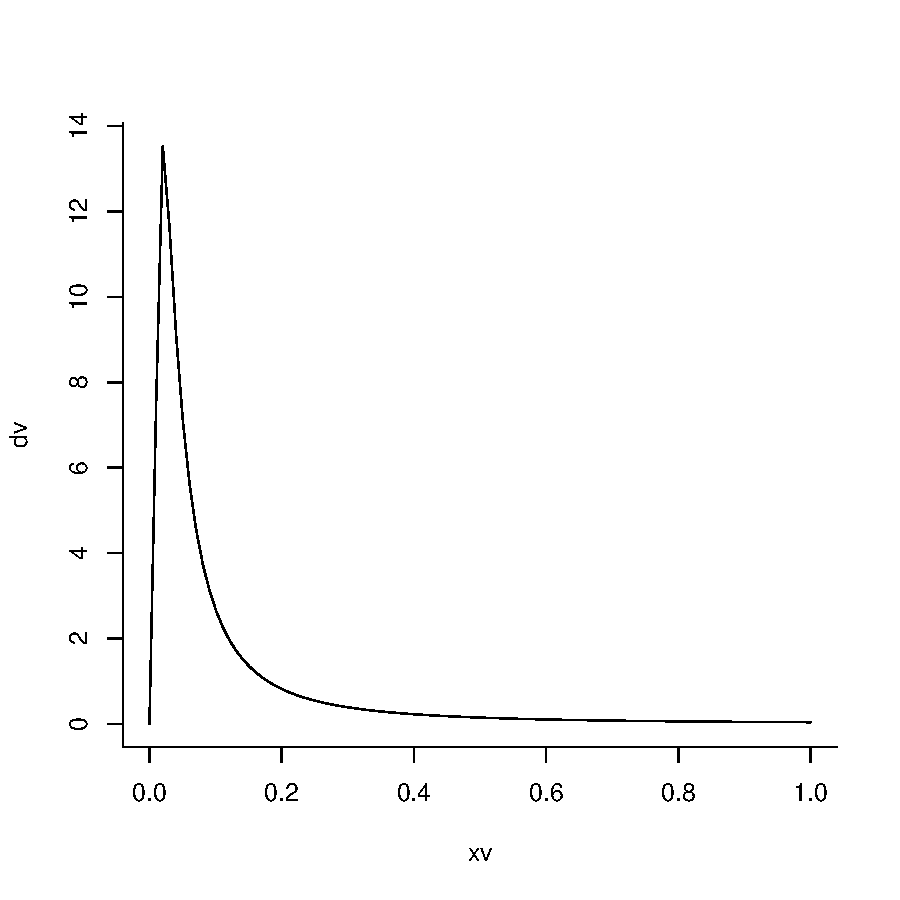
\includegraphics{Lecture3-028}
\end{center}
\caption{Marginal prior distribution of a variance using an inverse Wishart prior for the covariance matrix with \texttt{V=diag(3)*0.02} and \texttt{nu=4}.}
\label{NIc-fig}
\end{figure}


In Lecture \ref{chap2} we saw that a non-informative prior for a variance component was \texttt{V=0} and \texttt{nu=-2}. This result generalises to covariance matrices where the improper prior \texttt{V=diag(dim(V))$\ast$0} and \texttt{nu=dim(V)-3} is non-informative for the variances and covariances. This can be verified for the variances using the results derived above for the marginal distribution:

\begin{displaymath}
\begin{array}{rl}
\sigma^{2}_{1} \sim& IW\left(\texttt{nu}^{\ast}\texttt{=dim(V)-3-dim(V)+1},\ \texttt{V}^{\ast}=\frac{\texttt{nu}}{\texttt{nu}^{\ast}}\texttt{0}\right)\\
               \sim& IW\left(\texttt{nu}^{\ast}\texttt{=-2},\ \texttt{V}^{\ast}=\texttt{0}\right)\\

\end{array}
\end{displaymath}

\label{VCVprior-sec}
\ifalone
\end{document}
\else
\fi

